\documentclass[11pt, answers]{exam}
\renewcommand{\baselinestretch}{1.05}
\usepackage{amsmath,amsthm,verbatim,amssymb,amsfonts,amscd, graphicx}
\usepackage{graphics}

\usepackage{afterpage}
\usepackage{caption}

\usepackage{tikz}
\usepackage{fancybox}

\usepackage{clrscode3e}

\topmargin0.0cm
\headheight0.0cm
\headsep0.0cm
\oddsidemargin0.0cm
\textheight23.0cm
\textwidth16.5cm
\footskip1.0cm
\theoremstyle{plain}
\newtheorem{theorem}{Theorem}
\newtheorem{corollary}{Corollary}
\newtheorem{lemma}{Lemma}
\newtheorem{proposition}{Proposition}
\newtheorem*{surfacecor}{Corollary 1}
\newtheorem{conjecture}{Conjecture}  
\theoremstyle{definition}
\newtheorem{definition}{Definition}

 \begin{document}
 


\title{CSC263: Assignment 2}
\date{February 9th, 2017}
\author{Junjie Cheng, Jiayun Liu, Zi Hao Lin}
\maketitle

\unframedsolutions

\begin{questions}
\question
%Question1
\begin{solution}
\begin{parts}
\part 

\begin{minipage}[t]{\linewidth}
                \centering
\begin{tikzpicture}
[ 
level distance=9mm, 
every node/.style={circle, draw, inner sep=1.5pt},
level 1/.style={sibling distance=45mm}, 
level 2/.style={sibling distance=22mm}, 
level 3/.style={sibling distance=10mm},
level 4/.style={sibling distance=7mm},
label distance=-1mm
]

\node (root) [label=90:$-1$] {14} 
child {node[label=130:$+1$] {8} 
	child {node[label=130:$-1$] {7} 
		child {node[label=130:$0$] {6}} 
		child {missing}
	}
	child {node[label=50:$+1$] {10} 
		child {node[label=130:$0$] {9} 
		    child{missing}
		    child{missing}}
		child {node[label=50:$-1$] {12}
		    child{node[label=130:$0$] {11}}
		    child{missing}}
	} 
}
child {node[label=50:$+1$] {17}
 	child {node[label=130:$0$] {15} 
 		child {missing} 
 		child {missing}
 	}
 	child {node[label=50:$+1$] {19}
		child {missing}
		child {node[label=50:$0$] {21}}
	}
};
\end{tikzpicture}
\end{minipage}

\part 


\begin{minipage}[t]{\linewidth}
                \centering
\begin{tikzpicture}
[ 
level distance=9mm, 
every node/.style={circle, draw, inner sep=1.5pt},
level 1/.style={sibling distance=45mm}, 
level 2/.style={sibling distance=22mm}, 
level 3/.style={sibling distance=10mm},
level 4/.style={sibling distance=7mm},
label distance=-1mm
]

\node (root) [label=90:$0$] {10} 
child {node[label=130:$-1$] {8} 
	child {node[label=130:$-1$] {7} 
		child {node[label=130:$0$] {6}} 
		child {missing}
	}
	child {node[label=50:$0$] {9}
	} 
}
child {node[label=50:$0$] {14}
		child {node[label=130:$-1$] {12}
		    child{node[label=130:$0$] {11}}
		    child{missing}
 	}
 	child {node[label=50:$0$] {19}
		child {node[label=130:$0$] {15}}
		child {node[label=50:$0$] {21}}
	}
};
\end{tikzpicture}
\end{minipage}

\end{parts}

\end{solution}

\question
%Question2
\begin{solution}
\begin{parts}
\part 

Disprove: \\
Let T be: \\
\begin{minipage}[t]{\linewidth}
                \centering
\begin{tikzpicture}
[ 
level distance=9mm, 
every node/.style={circle, draw, inner sep=1.5pt},
level 1/.style={sibling distance=22mm}, 
level 2/.style={sibling distance=10mm}, 
label distance=-1mm
]

\node (root) [label=90:$+1$] {7} 
child {node[label=90:$0$] {3} 
    child{missing}
    child{missing}
}
child {node[label=90:$-1$] {11}
 	child {node[label=90:$0$] {9} 
 	}
    child {missing}
};
\end{tikzpicture}
\end{minipage}

Then $T'= \proc{$DELETE$}(T,3)$ will be: \\
\begin{minipage}[t]{\linewidth}
                \centering
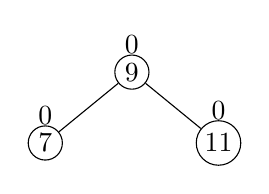
\begin{tikzpicture}
[ 
level distance=9mm, 
every node/.style={circle, draw, inner sep=1.5pt},
level 1/.style={sibling distance=22mm}, 
level 2/.style={sibling distance=10mm}, 
label distance=-1mm
]

\node (root) [label=90:$0$] {9} 
child {node[label=90:$0$] {7} 
}
child {node[label=90:$0$] {11}
};
\end{tikzpicture}
\end{minipage}

$T''= \proc{$INSERT$}(T',3)$ will be: \\
\begin{minipage}[t]{\linewidth}
                \centering
\begin{tikzpicture}
[ 
level distance=9mm, 
every node/.style={circle, draw, inner sep=1.5pt},
level 1/.style={sibling distance=22mm}, 
level 2/.style={sibling distance=10mm}, 
label distance=-1mm
]

\node (root) [label=90:$-1$] {9} 
child {node[label=90:$-1$] {7} 
    child{node[label=90:$0$] {3}}
    child {missing}
}
child {node[label=90:$0$] {11}
 	child {missing}
    child {missing}
};
\end{tikzpicture}
\end{minipage}

$T'' \neq T$. Hence statement disproved.

\part
Suppose T is a tree with 12 nodes:\\
\begin{minipage}[t]{\linewidth}
                \centering
\begin{tikzpicture}
[ 
level distance=9mm, 
every node/.style={circle, draw, inner sep=1.5pt},
level 1/.style={sibling distance=45mm}, 
level 2/.style={sibling distance=22mm}, 
level 3/.style={sibling distance=10mm},
level 4/.style={sibling distance=7mm},
label distance=-1mm
]

\node (root) [label=90:$-1$] {8} 
child {node[label=130:$-1$] {5} 
	child {node[label=130:$-1$] {3} 
		child {node[label=130:$-1$] {2}
		    child {node[label=130:$0$] {1}} 
		    child {missing}} 
		child {node[label=50:$0$] {4}} 
	}
	child {node[label=50:$-1$] {7} 
		child {node[label=130:$0$] {6}} 
		child{missing}
	} 
}
child {node[label=50:$-1$] {11}
 	child {node[label=130:$-1$] {10}
 	    child{node[label=130:$0$] {9}}
 	    child{missing}}
 	child {node[label=50:$0$] {12}	}
};
\end{tikzpicture}
\end{minipage}

Then we invoke $DELETE(T,12)$.\\
Immediately after the node is removed, we get\\

\begin{minipage}[t]{\linewidth}
                \centering
\begin{tikzpicture}
[ 
level distance=9mm, 
every node/.style={circle, draw, inner sep=1.5pt},
level 1/.style={sibling distance=45mm}, 
level 2/.style={sibling distance=22mm}, 
level 3/.style={sibling distance=10mm},
level 4/.style={sibling distance=7mm},
label distance=-1mm
]

\node (root) [label=90:$-1$] {8} 
child {node[label=130:$-1$] {5} 
	child {node[label=130:$-1$] {3} 
		child {node[label=130:$-1$] {2}
		    child {node[label=130:$0$] {1}} 
		    child {missing}} 
		child {node[label=50:$0$] {4}} 
	}
	child {node[label=50:$-1$] {7} 
		child {node[label=130:$0$] {6}} 
		child{missing}
	} 
}
child {node[label=50:$-2$] {11}
 	child {node[label=130:$-1$] {10}
 	    child{node[label=130:$0$] {9}}
 	    child{missing}}
 	child {missing}
};
\end{tikzpicture}
\end{minipage}

Node 11 is unbalanced. After the first rebalancing we have:\\
\begin{minipage}[t]{\linewidth}
                \centering
\begin{tikzpicture}
[ 
level distance=9mm, 
every node/.style={circle, draw, inner sep=1.5pt},
level 1/.style={sibling distance=45mm}, 
level 2/.style={sibling distance=22mm}, 
level 3/.style={sibling distance=10mm},
level 4/.style={sibling distance=7mm},
label distance=-1mm
]

\node (root) [label=90:$-2$] {8} 
child {node[label=130:$-1$] {5} 
	child {node[label=130:$-1$] {3} 
		child {node[label=130:$-1$] {2}
		    child {node[label=130:$0$] {1}} 
		    child {missing}} 
		child {node[label=50:$0$] {4}} 
	}
	child {node[label=50:$-1$] {7} 
		child {node[label=130:$0$] {6}} 
		child{missing}
	} 
}
child {node[label=50:$0$] {10}
 	child {node[label=130:$0$] {9}}
 	child {node[label=50:$0$] {11}	}
};
\end{tikzpicture}
\end{minipage}

Now Node 8 is unbalanced, so we need a second rebalancing:\\
\begin{minipage}[t]{\linewidth}
                \centering
\begin{tikzpicture}
[ 
level distance=9mm, 
every node/.style={circle, draw, inner sep=1.5pt},
level 1/.style={sibling distance=45mm}, 
level 2/.style={sibling distance=22mm}, 
level 3/.style={sibling distance=10mm},
level 4/.style={sibling distance=7mm},
label distance=-1mm
]

\node (root) [label=90:$0$] {5} 
child {node[label=130:$-1$] {3} 
	child {node[label=130:$-1$] {2} 
		child {node[label=130:$0$] {1}}
		child {missing} 
	}
	child {node[label=50:$0$] {4} 
		child{missing} 
		child{missing}
	} 
}
child {node[label=50:$0$] {8}
 	child {node[label=130:$-1$] {7}
 	    child{node[label=130:$0$] {6}}
 	    child{missing}}
 	child {node[label=50:$0$] {10}
 	    child{node[label=130:$0$] {9}}
 	    child{node[label=50:$0$] {11}}}
};
\end{tikzpicture}
\end{minipage}

\end{parts}
\end{solution}


\question
%Question3
\begin{solution}\\
The condition for a binary search tree to be balanced is that for each node, the height of the left sub-tree and the height of the right sub-tree differ by at most one.

The following is the algorithm.

\begin{codebox}
\Procname{$\proc{$AVL\_Balance\_Check$}(T)$}
\li \If $(\proc{$BF\_Check$}(T) == -1$)
\li     \Then \Return \proc{false}
\li \Else
\li     \Return \proc{true}
\end{codebox}

\begin{codebox}
\Procname{$\proc{$BF\_Check$}(T)$}
\li \If $(T == Nil)$ 
\li     \Then \Return $0$ //Base case
\li \Else
\li     $left \gets \proc{$BF\_Check$}(T.lchild)$
\li     $right \gets \proc{$BF\_Check$}(T.rchild)$
\li     \If $(left == -1 $ or $ right == -1)$ // Already unbalanced
\li         \Then \Return $-1$ 
\li     \ElseIf $(right - left == 1)$       // $BF=1$
\li         \Then \Return $right+1$ 
\li     \ElseIf $(right - left == 0)$       // $BF=0$
\li         \Then \Return $right+1$ 
\li     \ElseIf $(right - left == -1)$      // $BF=-1$
\li         \Then \Return $left+1$ 
\li     \Else // Unbalanced
\li         \Return $-1$ \End \End
\end{codebox}

The helper function $\proc{$BF\_Check$}(T)$ checks whether the binary search tree $T$ is an AVL tree. It returns $-1$ if the tree $T$ is unbalanced, otherwise, it returns the height of tree $T$ + 1.

First it check $T$'s sub-trees (we are treating $Nil$ as an "empty tree", which is vacuously an AVL tree). If either of $T$'s sub-tree is not an AVL tree, T cannot be an AVL tree. $-1$ is returned.

Also, to satisfy the AVL balancing condition, the difference between the height of $T$'s left sub-tree (i.e. the return value of $\proc{$BF\_Check$}(T.left)-1$, if it is balanced) and the height of $T$'s right sub-tree (i.e. the return value of $\proc{$BF\_Check$}(T.right)-1$, if it is balanced) must be at most 1. In these cases, the height of tree $T + 1$ is returned. 

If the difference between the heights of the sub-trees of $T$ is greater than $1$, then $T$ does not satisfy the AVL balancing condition, and $-1$ is returned.

The function $\proc{$AVL\_Balance\_Check$}(T)$ translate the result of $\proc{$BF\_Check$}(T)$ into $TRUE$ or $FALSE$ according to its return value.
\begin{itemize}
\item Worst-case running time
\end{itemize}
The helper function $\proc{$BF\_Check$}(T)$ has a worst case running time of $\Theta(n)$, where $n$ is the number of the nodes in the tree $T$.

First, by line 4 and line 5, both left sub-tree and right sub-tree are called (for all non-empty trees). Because of the recursion, every node in tree $T$ is called exactly once, and all the (imaginary) empty "sub-trees" of leaves and one-child nodes are called exactly once.

In the worst case (in fact, in any case), there will be a total of $n+1$ such empty "sub-trees". The proof is easy. Let's create a new tree, $T^*$, by making all "empty nodes" in tree $T$ "real nodes". Then, all of the "empty nodes" become the leaves in $T*$, and all nodes originally in $T$ becomes internal nodes in $T^*$. Note that $T^*$ is a full (or proper/plane) binary tree (that is, every node in the tree has either 0 or 2 children). So, the number of "empty nodes" in $T$, should be the total number of the leaves in $T^*$, which, according to the property of full binary tree, should equal the number of internal nodes in the tree $T^*$ $+1$, i.e. $n+1$.

For each of the "empty node", function $\proc{$BF\_Check$}()$ executes only one comparison before returning. A total of $n+1$ comparisons are made for all "empty nodes".

For each of the "internal nodes" of $T^*$ (i.e. the nodes of $T$), from line 1 to 5, 1 comparison and 2 assignments must be executed. In the worst case, there can be at most 5 more comparisons, executed on line 6, 6, 8, 10, 12 successively. So, in the worst case, 2 assignments and 6 comparisons are made for each node in tree $T$, resulting a total of $6n$ comparisons and $2n$ assignments.

Using $c$ to denote the time for each comparison and $a$ to denote the time for each assignment, the time complexity of $\proc{$BF\_Check$}(T)$ is $$(n+1)c+6nc+2na == 7nc+c+2na$$. Note that $\proc{$AVL\_Balance\_Check$}(T)$ performs one $\proc{$BF\_Check$}(T)$ function all and one comparison, the time complexity of $\proc{$AVL\_Balance\_Check$}(T)$ is $$T(n) = 7nc+2c+2na$$.
Note that there exist positive constant$c_1=2a+7c$, $c_2=2a+9c$, $n_0=2$ such that $$\forall n\geq n_0 .\  0\leq c_1n \leq T(n) \leq c_2n$$
So, $$T(n) \in \Theta(n)$$, i.e. the time complexity of the algorithm is in $\Theta(n)$.
\end{solution}

\question
%Question4
\begin{solution}
\begin{enumerate}
\item The data structure we are using is AVL tree. \\
The tree will store m (or the number of inputs so far, whichever is smaller) smallest values of all the inputs so far.

\item The algorithm is, insert the first $m$ input values into the AVL tree directly, so that the tree gets a size of $m$. Then, for each of following inputs, say, $input$, compare $input$ with the largest element$^1$, say, $l$, in the AVL tree. If $input$ is less than $l$, then delete $l$ from the tree and then add $input$ to the AVL tree; else, do nothing$^2$. When a query is requested, do an inorder tree traversal$^3$ and print each value.

Notes: 
1. The largest element is obtained by traversing along the right child all the way down the tree.

2. This ensures that the elements in the AVL tree are the smallest $m$ values of all the inputs. 

3.  According to the property of AVL tree, the inorder traversal will visit the nodes in the order that the data of the nodes are increasing.

\item The following is the pseudo-code.
Initial values for global variables:
\begin{codebox}
\li (int) count=0
\li (AVL\_Tree) T=Nil
\end{codebox}

\begin{codebox}
\Procname{$\proc{$Input$}(input, m)$}
\li \If $(input == query)$ \\// The question assumes there are already enough inputs when query is called.
\li     \Then $\proc{$In\_Order\_Print$}(T)$
\li     \Else
\li     \If $(count < m)$ // Less than m inputs given
\li         \Then $\proc{$AVL\_Insert$}(T, input)$
\li         count++
\li     \Else // At least m inputs given; $T$ is not empty
\li         $l \gets \proc{$Max\_Value$}(T)$
\li         \If $(input<x)$
\li             \Then $\proc{$AVL\_Delete$}(T, l)$
\li             $\proc{$AVL\_Insert$}(T, input)$
\end{codebox}
Helper functions:
\begin{codebox}
\Procname{$\proc{$Max\_Value$}(T)$}
\li \While $(T.right)$ // Note that $T$ cannot be an empty tree, so $T$ has the attribute $right$.
\li     \Do $T \gets T.right$ \End
\li \Return $T.key$
\end{codebox}
\begin{codebox}
\Procname{$\proc{$In\_Order\_Print$}(T)$}
\li \If $(T.left)$
\li     \Then $\proc{$In\_Order\_Print$}(T.left)$ \End
\li print $(T.key)$
\li \If $(T.right)$
\li     \Then $\proc{$In\_Order\_Print$}(T.right)$ \End
\end{codebox}
Pseudo-code for $\proc{$AVL\_Insert$}()$ and $\proc{$AVL\_Delete$}()$ is in the handout.

\item 
\begin{itemize}
\item Time complexity for processing input key:

When processing a key, the condition in line 1 is always evaluated as false (evaluation taking $O(1)$ time), so the else block from line 3 to 11 is executed.

(Special case) Initiation of global variables takes $O(1)$ time, we count this as part of the operation to process the first input key.
In fact, processing the first input takes only $O(1)$ time. Line 4 condition must be true, and what line 5 does is actually creating an AVL Node with $key=input$ and pointing $T$ to that node, which takes constant time. Addition in line 6 also takes constant time. So, first key process takes $O(1)$ time.

For the following inputs, 

(Case i) if the condition in line 4 is true, then $O(\log{(sizof(T))}$ time is taken on line 5 and constant time is taken on line 6. Note that $sizeof(T) =count< m$, so the total time taken is bounded above by $O(1)+O(\log{m})+O(1)=O(\log{m})$. 

(Case ii) If the condition in line 4 is false, then, $T$ is already of $m$. In the worst case, the condition in line 9 is true and line 8, 10, 11 are executed. The function $\proc{$Max\_Value$}(T)$ in line 8, traverses along the path to the right-most leaf. 
Note that the height of an AVL tree with $m$ nodes, in the worst case, is $1.44\log_2{(m+2)}\in O(\log{m})$, so at most $O(\log{m}+1)$ nodes are visited. Also note that on each node, the code runs a constant time, line 8 runs $O(\log{m}+1))*O(1) = O(\log{m})$ time.
$\proc{$AVL\_Insert$}()$ and $\proc{$AVL\_Delete$}()$, according to the handout, can be done in $O(\log{m})$ time. So, the worst case running time for (Case ii) is $O(1)+O(\log{m})+O(\log{m}) = O(\log{m})$ time, same as (Case i).

Thus, in the worst case, processing a input key takes $O(\log{m})$ time.

\item Time complexity for processing query:
When query is the input, only line 1 (constant time comparison) and line 2 are executed. Note that at least $m$ keys are input, so the AVL tree $T$ must has a size of $m$. For each node, the function $\proc{$In\_Order\_Print$}(T)$ will check the existence of left and right child and visit every existing child. So every node in the tree is visited once. On each visit, the function makes 2 comparisons and 1 print, which takes constant time. Thus, the function takes $O(m) * O(1)=O(m)$ time.
\end{itemize}
\end{enumerate}

\end{solution}

\end{questions}



\end{document}
